\documentclass[tikz,border=6pt]{standalone}
\usepackage{xcolor}
\usetikzlibrary{arrows.meta}

\definecolor{lineblue}{HTML}{4A90D9}
\definecolor{linegray}{HTML}{333333}

\begin{document}
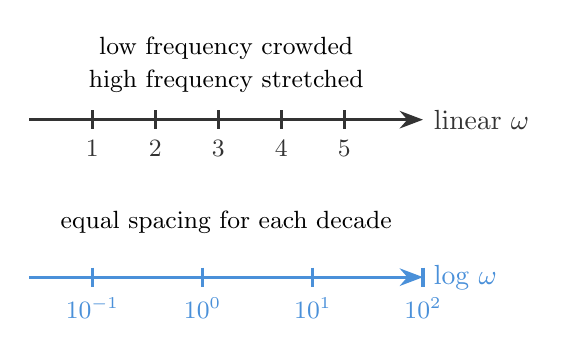
\begin{tikzpicture}[line width=1.2pt, >=Stealth]
  \draw[linegray, ->] (0,0) -- (5,0) node[right] {linear $\omega$};
  \foreach \x/\t in {0.8/1,1.6/2,2.4/3,3.2/4,4.0/5}{
    \draw[linegray] (\x,0.12) -- (\x,-0.12) node[below] {\small \t};
  }
  \node[align=center] at (2.5,0.7) {\small low frequency crowded\\\small high frequency stretched};

  \draw[lineblue, ->] (0,-2.0) -- (5,-2.0) node[right] {log $\omega$};
  \foreach \x/\t in {0.8/$10^{-1}$,2.2/$10^0$,3.6/$10^1$,5.0/$10^2$}{
    \draw[lineblue] (\x,-1.88) -- (\x,-2.12) node[below] {\small \t};
  }
  \node[align=center] at (2.5,-1.3) {\small equal spacing for each decade};
\end{tikzpicture}
\end{document}
